% Horizon- and Regime-Adaptive Weighted Ensemble Forecasting of Urban Crime
% Target: Neural Computing and Applications (Springer). First draft.
% Standalone-compilable (article class); port to Springer sn-jnl.cls before submission.
% TODO: confirm author names/order/affiliations and ORCID.
\documentclass[11pt]{article}
\usepackage[utf8]{inputenc}
\usepackage{amsmath,amssymb}
\usepackage{graphicx}
\graphicspath{{../figures/}}
\usepackage{booktabs}
\usepackage{array}
\usepackage[hidelinks]{hyperref}
\usepackage[margin=1in]{geometry}
\usepackage{authblk}

\title{Horizon- and Regime-Adaptive Weighted Ensemble Forecasting of Urban Crime:
When and Where Does Adaptivity Pay?}
\author[1]{Felicia Sword}
\author[1]{Christopher Andreas}
\affil[1]{\small TODO: Department, Institution, City, Country. \texttt{felicia.sword@gmail.com}}
\date{}

\begin{document}
\maketitle

\begin{abstract}
Short-term, district-level crime forecasting supports patrol and resource planning, but
existing ensemble approaches typically \emph{compare} forecasters or apply a single fixed
weight vector, leaving untested \emph{when} combining helps and whether the optimal model
mix is stable across forecast horizon and across structural change. We forecast weekly total
incident counts for 22 Chicago police districts (2015--2026) at horizons of 1, 4, 8 and 12
weeks using five base learners---seasonal-naive, SARIMA, Prophet, a global gradient-boosting
model (XGBoost) and a global recurrent neural network (LSTM)---and three weighting schemes:
a static inverse-RMSE blend, a horizon-adaptive blend with a separate constrained weight
vector per horizon, and a regime-adaptive blend that re-estimates weights on a rolling
window. All weights are fit on a validation split only, and forecasts are produced by a
strictly temporal rolling-origin backtest. The ensemble significantly outperforms the best
single model at every horizon (Diebold--Mariano, $p<0.05$), with the advantage growing from
roughly 2\% at one week to 12\% at twelve weeks. The optimal weights demonstrably shift with
horizon, and---using a split that places the 2020 COVID-19 structural break inside the test
window---we show the advantage of adaptive over static weighting concentrates exactly at the
regime change: the regime-adaptive blend improves on the static blend by 7--11\% during the
acute shock versus approximately 0\% in calm periods. SHAP analysis of the gradient-boosting
member shows its drivers shift from recent momentum at short horizons to seasonality at long
horizons, mirroring why the optimal mix changes. The central finding is that the optimal
forecaster mix is not constant, and that the value of adaptivity is \emph{conditional} on
regime change.
\end{abstract}

\noindent\textbf{Keywords:} crime forecasting; time-series ensemble; adaptive weighting;
forecast combination; Diebold--Mariano test; structural break; SHAP.

\section{Introduction}
Reported crime in large cities is logged at scale---Chicago's open data portal records
roughly eight million incidents since 2001---and accurate short-term forecasts of district-level
workload support patrol allocation and resource planning. Weekly district counts are nonetheless
hard to forecast: they exhibit strong yearly seasonality, a long-run decline, and a sharp
structural break in 2020 associated with the COVID-19 pandemic.

A large body of recent work forecasts crime with ensembles of statistical and machine-learning
models (e.g., SARIMA, Prophet, gradient boosting and deep networks). This template is now
saturated, and existing studies generally either \emph{compare} models and select a winner, or
combine them with a single fixed weight vector. Two questions remain under-tested. First,
\emph{when} does combining help---at which horizons, and against which baselines? Second, is the
optimal model mix \emph{stable}, or does it shift with the forecast horizon and with the
data-generating regime?

We address these questions directly. Our contribution is a \emph{mechanism and a finding}, not a
new assembly of off-the-shelf models:
\begin{enumerate}
  \item A \textbf{horizon- and regime-adaptive weighted ensemble} that re-estimates member
  weights per forecast horizon and on a rolling window. The member set includes a deep-learning
  (LSTM) model, which we \emph{adaptively weight} rather than merely compare.
  \item Evidence that the optimal mix is \textbf{not constant}: the weight ordering changes with
  horizon, and authority re-allocates across the 2020 break. These ``weights versus horizon/time''
  results are findings, not incidental metrics.
  \item An \textbf{honest evaluation}: a mandatory seasonal-naive floor, Diebold--Mariano (DM)
  significance tests per horizon, and the mean absolute scaled error (MASE). We explicitly report
  where adaptive weighting does \emph{not} beat a simple static blend.
\end{enumerate}

We answer three research questions. \textbf{RQ1}: among the base models, which best forecasts
next-week district counts, and does the ranking hold at 4/8/12 weeks? \textbf{RQ2}: does a
weighted ensemble beat the best single model across horizons (DM), and does horizon-/regime-adaptive
weighting beat a static inverse-RMSE blend? \textbf{RQ3}: how do the optimal model and weights shift
across the 2020 regime break and across districts---is adaptivity the source of any gain?

\section{Related Work}
\textbf{Statistical and ML crime forecasting.} Classical approaches use ARIMA/SARIMA and, more
recently, Prophet and gradient boosting. The closest prior art to ours is a comparative study in
this journal that evaluates SARIMA, Prophet, HWES, LSTM and BLSTM (and several classifiers) across
San Francisco, Chicago and Philadelphia~\cite{ncaa2025}. Crucially, that work \emph{compares}
models; it does not combine them with adaptive weights, does not test forecast-combination
significance, and does not analyse the 2020 regime change. Our delta is precisely the adaptive
\emph{weighted} combination (including the deep-learning member), DM significance, the regime
analysis and member-level interpretability.

\textbf{Spatiotemporal deep learning.} Graph and attention-based spatiotemporal networks define the
state of the art on raw accuracy. We do not compete on that axis; we focus on \emph{adaptivity and
robustness under distribution shift}, which those models do not test, and we discuss this choice in
Section~\ref{sec:disc}.

\textbf{Forecast combination.} Combining forecasts is a classical idea; inverse-error weighting is a
standard, hard-to-beat baseline, and constrained optimal and time-varying weights have a long
history. We contribute a horizon- and regime-conditioned treatment on district-level crime, and a
characterisation of when each scheme wins.

\textbf{Global vs.\ local forecasting.} For many related series, a single global model that learns
across series can beat per-series local models~\cite{monteromanso2021}. We adopt this for the
XGBoost and LSTM members (district as a feature), reserving per-series fitting for SARIMA and Prophet.

\section{Data and Study Area}
We use the City of Chicago ``Crimes 2001--Present'' dataset (\texttt{ijzp-q8t2})~\cite{chicago}.
We aggregate incidents to weekly total counts per police district and restrict to the 22 active
districts and the modeling window 2015--2026. Absent week-buckets are true zeros and are filled as
zero (missing $\neq$ deleted); at the district-total level counts never reach zero (minimum
$\approx$52/week), so percentage errors remain well behaved. Exploratory analysis (Fig.~\ref{fig:eda})
confirms a long-run decline, strong summer seasonality, and a pronounced 2020 break
($-18.7\%$ year-on-year; an April-2020 trough). We use a strictly temporal split: training through
2020, validation 2021--2022, and test 2023 onward. For the regime study we additionally use a split
shifted three years earlier (training through 2018, validation 2019, test 2020--2022) so that the
2020 break falls inside the test window.

\begin{figure}[t]\centering
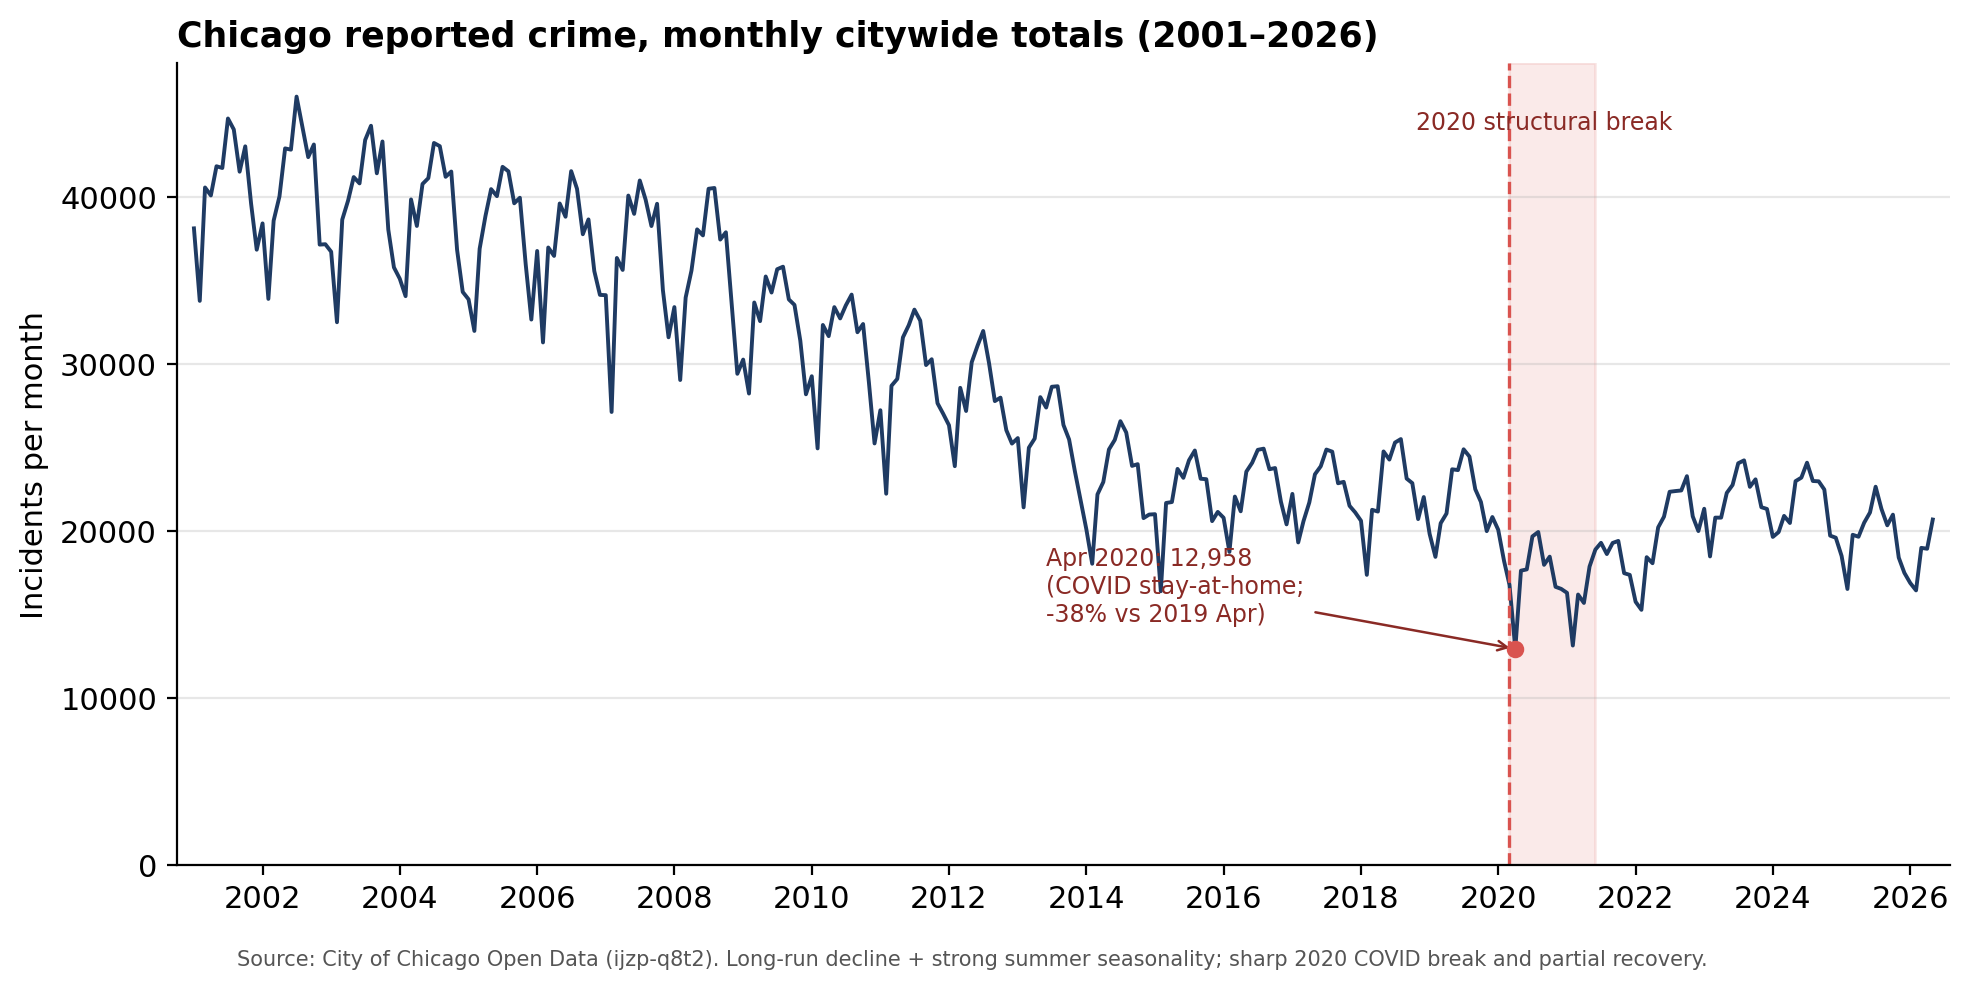
\includegraphics[width=0.82\linewidth]{fig1_monthly_overview.png}
\caption{Monthly citywide reported crime, 2001--2026; the 2020 COVID structural break (shaded) is the
central robustness stress-test. District-level profiles and spatial maps are provided as supplementary
EDA figures.}
\label{fig:eda}
\end{figure}

\section{Methodology}
\subsection{Problem formulation}
We forecast with a \emph{direct} multi-horizon strategy: for each horizon $h\in\{1,4,8,12\}$ weeks we
predict the count $h$ steps ahead from features computed at the origin week. Features are
leakage-safe: lags $\{1,2,3,4,8,12,52\}$, rolling mean/std over $\{4,8,12\}$ weeks, calendar terms,
a US-holiday flag, a COVID-window indicator, and the district identifier. All features use only
information available at the origin.

\subsection{Base learners}
\begin{itemize}
  \item \textbf{Seasonal-naive} (mandatory floor): $\hat{y}(t{+}h)=y(t{+}h{-}52)$.
  \item \textbf{SARIMA}: \texttt{auto\_arima} fitted per district (weekly seasonality $m{=}52$;
  orders cached, rolled forward).
  \item \textbf{Prophet}: per district, with yearly seasonality, US holidays, and a COVID regressor.
  \item \textbf{XGBoost}: a single \emph{global} gradient-boosting model across all districts (district
  as a feature).
  \item \textbf{LSTM}: a single \emph{global} recurrent network taking a standardized 52-week window of
  past counts, one model per horizon.
\end{itemize}

\subsection{Adaptive weighted ensemble}
The ensemble blends the four learning members $m\in\{$SARIMA, Prophet, XGBoost, LSTM$\}$ with
constrained weights $w_m\ge 0,\ \sum_m w_m=1$ (seasonal-naive is the baseline, not a member). We
compare three schemes:
\begin{enumerate}
  \item \textbf{Static inverse-RMSE} (baseline): one weight vector for all horizons, $w_m\propto
  1/\mathrm{RMSE}_m$ on validation.
  \item \textbf{Horizon-adaptive}: a separate constrained weight vector per horizon, minimising
  validation RMSE at that horizon (SLSQP).
  \item \textbf{Regime-adaptive}: weights re-estimated on a trailing 52-week window of already-realised
  errors, yielding time-varying weights.
\end{enumerate}
Weights are fit on the validation split only; the regime-adaptive scheme uses only past realised
errors at each origin (no future leakage).

\subsection{Backtest and evaluation}
A strictly temporal rolling-origin backtest emits forecasts keyed by (district, horizon, origin) so
every scheme is judged on identical points. We report MAE and RMSE (primary), MAPE/SMAPE (masked at
actual $=0$), and MASE scaled by the in-sample seasonal-naive. Statistical significance uses the
Diebold--Mariano test with the Harvey--Leybourne--Newbold small-sample correction and a squared-error
loss differential averaged across districts per origin week. We interpret the XGBoost member with SHAP
values (computed via the model's native TreeSHAP), framed as explaining that component, not the
ensemble.

\section{Results}
\subsection{Base-model comparison across horizons (RQ1)}
Table~\ref{tab:metrics} reports test-set error by horizon. XGBoost is the strongest single model
overall, with the LSTM competitive at short horizons; all learning models comfortably beat the
seasonal-naive floor (MASE $<1$, supporting H5), and errors grow with horizon.

\begin{table}[t]\centering
\caption{Test RMSE (left) and MASE (right) by forecast horizon (weeks), main split (test 2023+).
Lower is better; MASE $<1$ beats the seasonal-naive floor. Best in each column in \textbf{bold}.}
\label{tab:metrics}
\small
\begin{tabular}{l rrrr c rrrr}
\toprule
 & \multicolumn{4}{c}{RMSE} & & \multicolumn{4}{c}{MASE}\\
\cmidrule(lr){2-5}\cmidrule(lr){7-10}
Model & 1 & 4 & 8 & 12 & & 1 & 4 & 8 & 12\\
\midrule
Seasonal-naive      & 35.11 & 34.58 & 34.35 & 34.39 & & 0.95 & 0.94 & 0.93 & 0.93\\
SARIMA              & 26.28 & 27.25 & 28.35 & 28.84 & & 0.71 & 0.73 & 0.76 & 0.78\\
Prophet             & 27.26 & 27.08 & 27.94 & 28.96 & & 0.74 & 0.75 & 0.77 & 0.81\\
XGBoost             & 23.15 & 25.95 & 27.52 & 28.66 & & 0.64 & 0.71 & 0.74 & 0.77\\
LSTM                & 23.73 & 26.20 & 27.54 & 30.32 & & 0.64 & 0.70 & 0.74 & 0.82\\
\midrule
Static inv-RMSE     & 22.40 & \textbf{23.55} & \textbf{24.36} & \textbf{24.88} & & 0.61 & \textbf{0.64} & \textbf{0.66} & \textbf{0.68}\\
Horizon-adaptive    & \textbf{22.45} & 24.00 & 24.73 & 26.05 & & \textbf{0.61} & 0.64 & 0.66 & 0.70\\
Regime-adaptive     & 22.48 & 23.70 & 24.63 & 25.20 & & 0.61 & 0.64 & 0.66 & 0.68\\
\bottomrule
\end{tabular}
\end{table}

\subsection{Ensemble vs.\ best single model (RQ2)}
All three ensembles significantly outperform the best single model (XGBoost) at every horizon
(Diebold--Mariano, $p<0.05$; Table~\ref{tab:dm}), and the relative gain grows with horizon (from
$\approx$2\% at $h{=}1$ to $\approx$12\% at $h{=}12$), supporting H1. The differences \emph{among}
ensembles are small: in the calm 2023+ test period the static inverse-RMSE blend is statistically
indistinguishable from---and at long horizons marginally better than---the adaptive schemes. We report
this honestly; the value of adaptivity emerges under regime change (Section~\ref{sec:regime}).

\begin{table}[t]\centering
\caption{Diebold--Mariano tests (squared error, HLN correction), main split. Negative statistic
favours the ensemble; $^\ast$ denotes $p<0.05$.}
\label{tab:dm}
\small
\begin{tabular}{l rrrr}
\toprule
Comparison (per horizon) & 1 & 4 & 8 & 12\\
\midrule
Regime-adaptive vs.\ XGBoost & $-2.65^\ast$ & $-5.28^\ast$ & $-4.15^\ast$ & $-3.57^\ast$\\
Horizon-adaptive vs.\ XGBoost & $-2.46^\ast$ & $-4.54^\ast$ & $-5.65^\ast$ & $-5.05^\ast$\\
Static vs.\ XGBoost & $-2.85^\ast$ & $-6.45^\ast$ & $-4.73^\ast$ & $-3.77^\ast$\\
\bottomrule
\end{tabular}
\end{table}

\subsection{The optimal mix shifts with horizon (H2)}
Table~\ref{tab:weights} shows the horizon-adaptive weights. The mix is clearly not constant: the LSTM
receives substantial weight at short horizons (0.36 at $h{=}1$, 0.47 at $h{=}4$) but is driven to zero
at $h{=}12$, where XGBoost dominates (0.66). The ensemble thus uses the deep-learning member precisely
where it is competitive and discards it where it is not---an illustration of the mechanism.

\begin{table}[t]\centering
\caption{Horizon-adaptive ensemble weights (fit on validation), main split.}
\label{tab:weights}
\small
\begin{tabular}{l rrrr}
\toprule
Horizon (wk) & SARIMA & Prophet & XGBoost & LSTM\\
\midrule
1  & 0.32 & 0.08 & 0.24 & 0.36\\
4  & 0.31 & 0.01 & 0.22 & 0.47\\
8  & 0.24 & 0.10 & 0.50 & 0.17\\
12 & 0.28 & 0.07 & 0.66 & 0.00\\
\bottomrule
\end{tabular}
\end{table}

\subsection{The 2020 regime break (RQ3)}\label{sec:regime}
Using the shifted split that places 2020 in the test window, Fig.~\ref{fig:traj} shows the
regime-adaptive weights over time. Authority re-allocates sharply across the break: the ensemble
shifts almost entirely to Prophet during the acute COVID shock, then returns weight to XGBoost and the
LSTM in recovery, with SARIMA re-emerging in 2022. Table~\ref{tab:regime} quantifies the payoff: the
regime-adaptive blend improves on the static blend by 7--11\% during the acute shock, but by
approximately 0\% (occasionally slightly negative) in the calm recovery. The improvement is
statistically significant at $h{=}1$ within the acute-shock window ($p=0.041$). This supports H3 in
the form the data warrant: \emph{adaptivity's advantage is conditional on regime change}, and it is
largest precisely at the structural break.

\begin{figure}[t]\centering
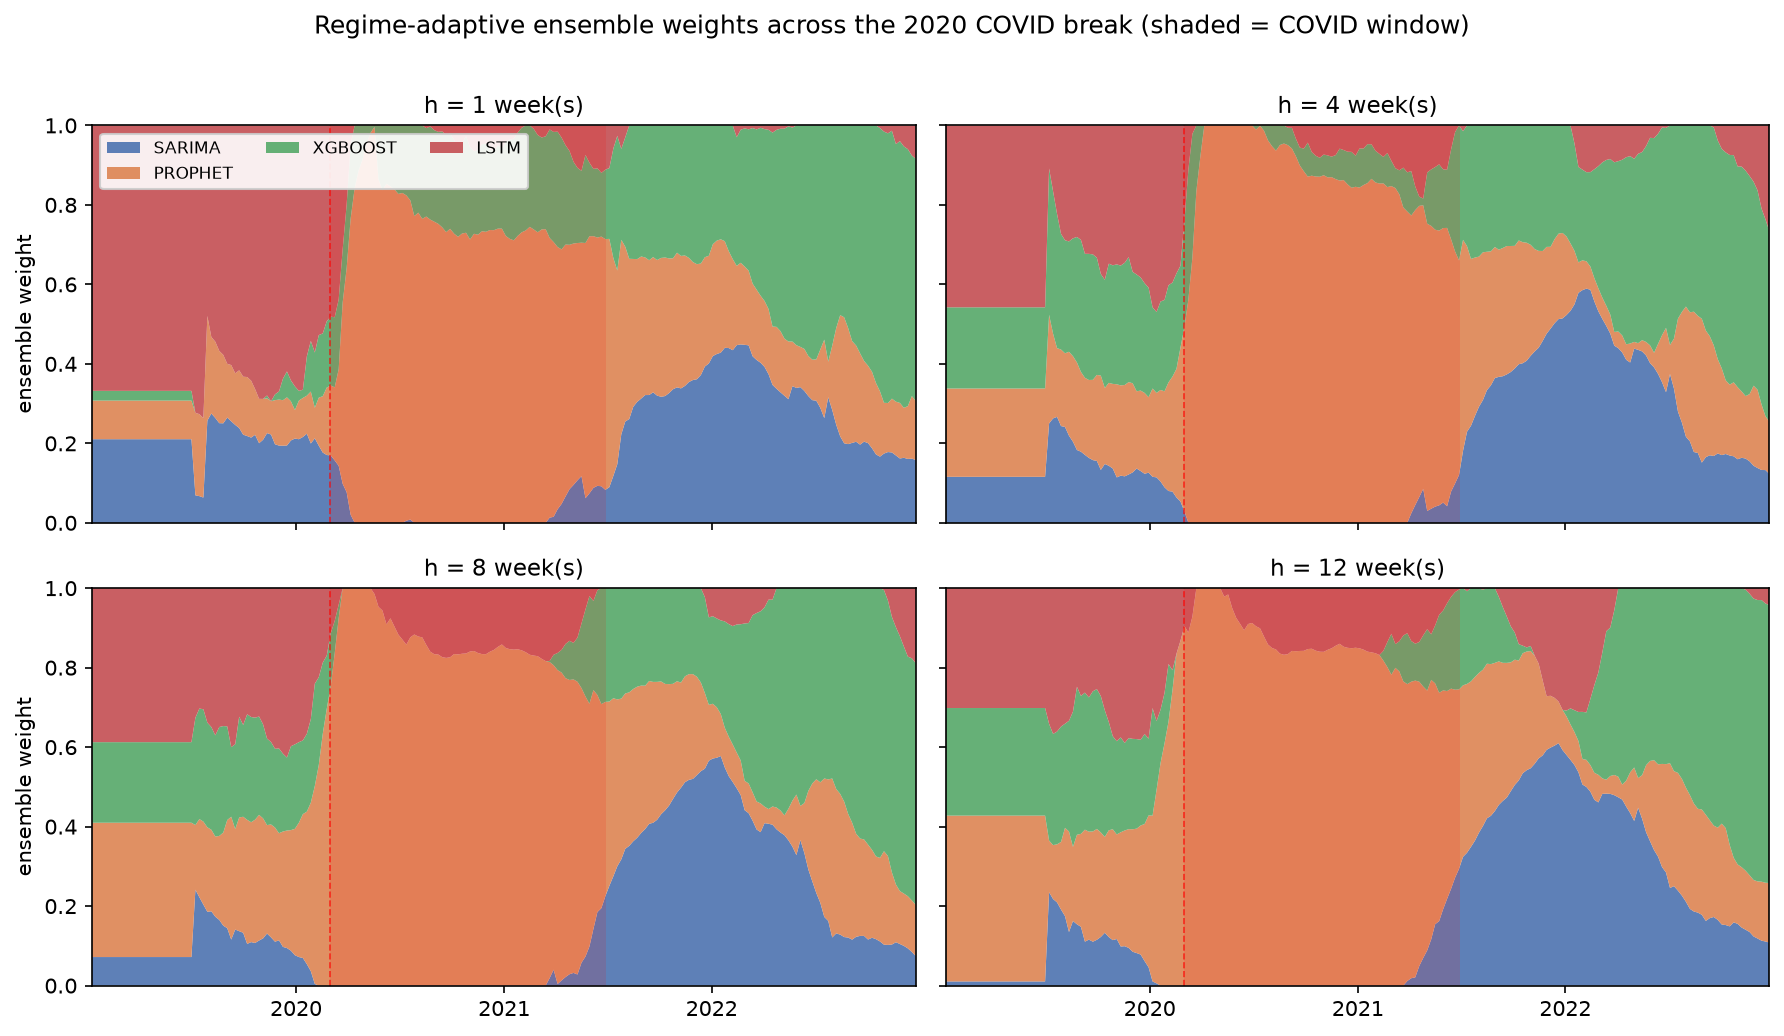
\includegraphics[width=\linewidth]{fig_weight_trajectory_2020.png}
\caption{Regime-adaptive ensemble weights across the 2020 COVID break (shaded = COVID window), per
horizon. Authority re-allocates from a balanced mix to Prophet during the shock, then reverts.}
\label{fig:traj}
\end{figure}

\begin{table}[t]\centering
\caption{Regime-adaptive improvement over the static blend (\% RMSE), by regime window and horizon.}
\label{tab:regime}
\small
\begin{tabular}{l rrrr}
\toprule
Window & 1 & 4 & 8 & 12\\
\midrule
Pre-shock (2020 Jan--Feb) & 0.8 & 0.4 & 2.5 & 4.4\\
Acute shock (2020-03--2021-06) & \textbf{7.4} & \textbf{9.7} & \textbf{10.2} & \textbf{10.6}\\
Recovery (2021-07--2022-12) & $-1.2$ & $-1.4$ & 1.2 & 0.5\\
\bottomrule
\end{tabular}
\end{table}

\subsection{Per-district heterogeneity (H4)}
The ensemble helps in 18 of 22 districts (mean gain $\approx$8\% RMSE over the best single model), but
the gain does \emph{not} scale with district volatility (Spearman $\rho=0.17$, $p=0.44$;
Fig.~\ref{fig:h4}). We therefore do \emph{not} find support for H4: gains are pervasive but not
concentrated in high-volatility districts.

\begin{figure}[t]\centering
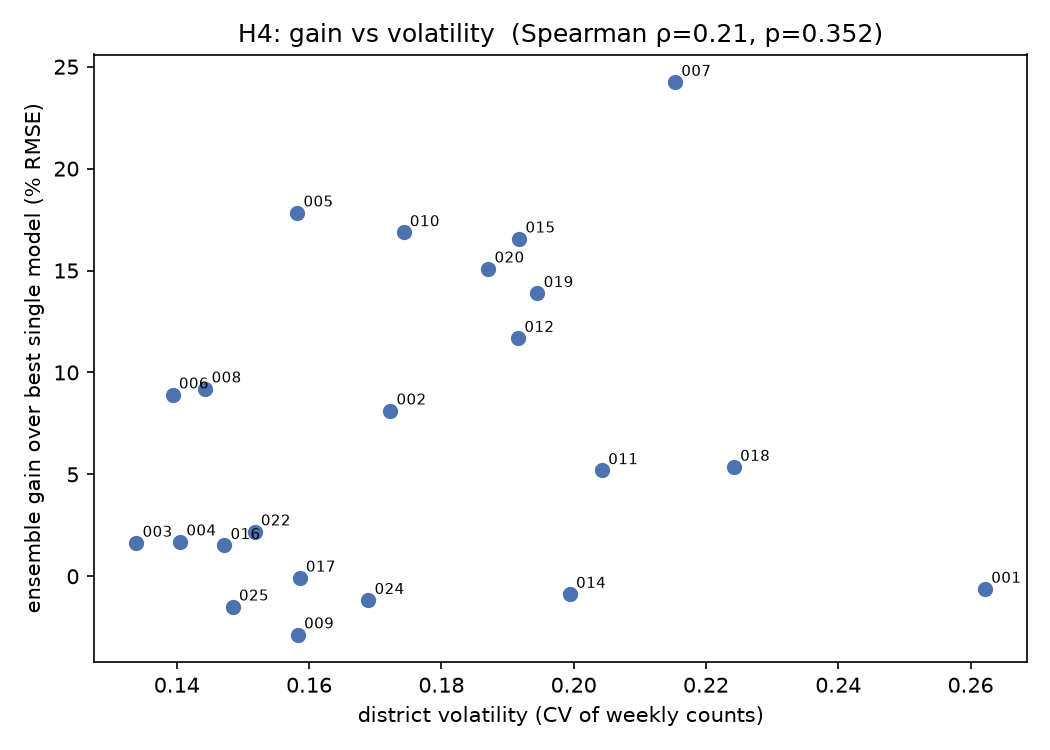
\includegraphics[width=0.7\linewidth]{fig_h4_gain_vs_volatility.png}
\caption{Per-district ensemble gain over the best single model versus district volatility (coefficient
of variation of weekly counts). The relationship is weak and non-significant (H4 not supported).}
\label{fig:h4}
\end{figure}

\subsection{Robustness}
Across ten random seeds the ensemble's test RMSE is highly stable (standard deviation 0.02--0.12), and
the ensemble is more stable than the XGBoost member alone---combination reduces variance. Conclusions
are also robust to the training-window length (starting the XGBoost member's training in 2015, 2017 or
2019 changes test RMSE only marginally).

\subsection{Interpretability (SHAP)}
SHAP values for the XGBoost member (Figs.~\ref{fig:shapsum} and \ref{fig:shaph}) show its drivers
shift with horizon: short-horizon forecasts are dominated by recent rolling means (momentum), whereas
at twelve weeks calendar and seasonal features (month, week-of-year) become the largest contributors.
This mirrors, at the member level, why the optimal ensemble mix changes with horizon.

\begin{figure}[t]\centering
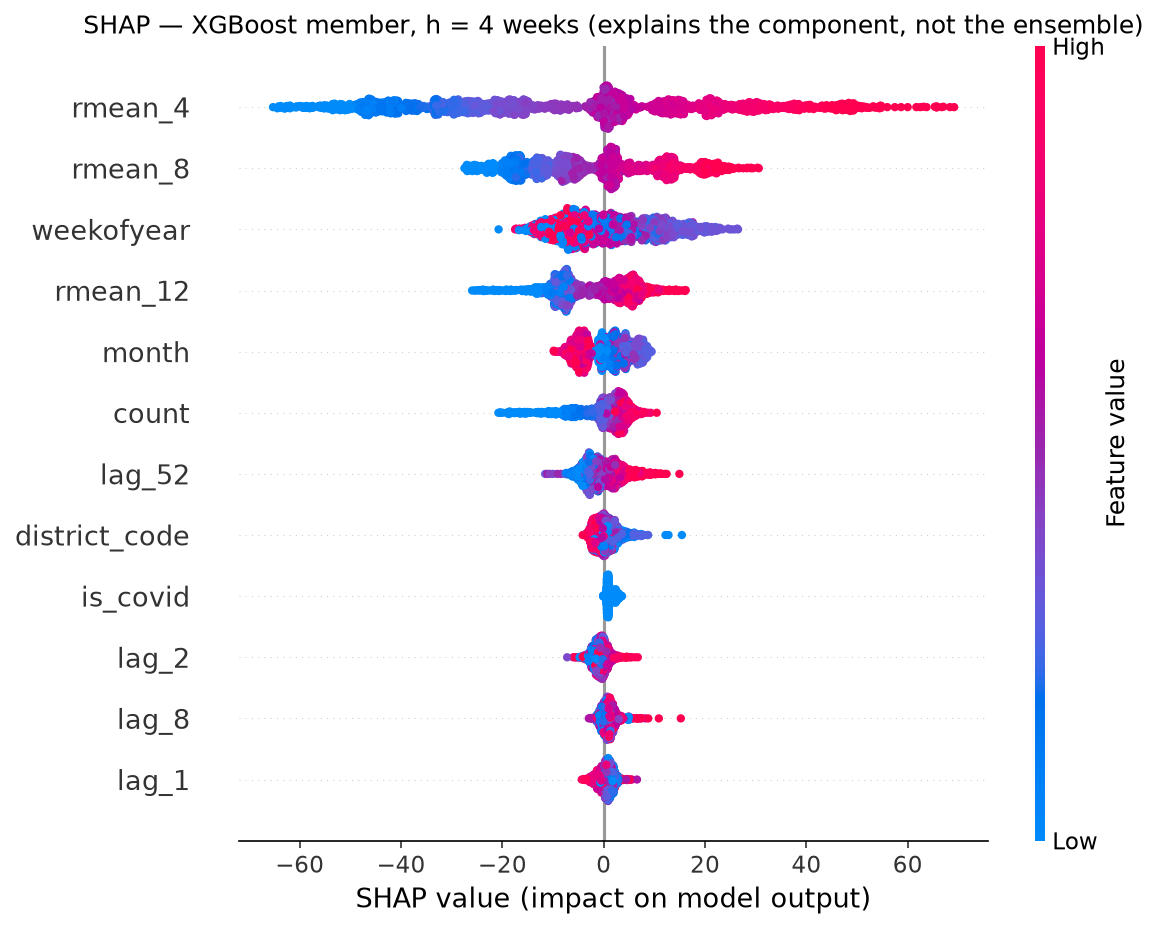
\includegraphics[width=0.78\linewidth]{fig_shap_summary.png}
\caption{SHAP summary (beeswarm) for the XGBoost member at a representative horizon, explaining that
component (not the ensemble).}
\label{fig:shapsum}
\end{figure}

\begin{figure}[t]\centering
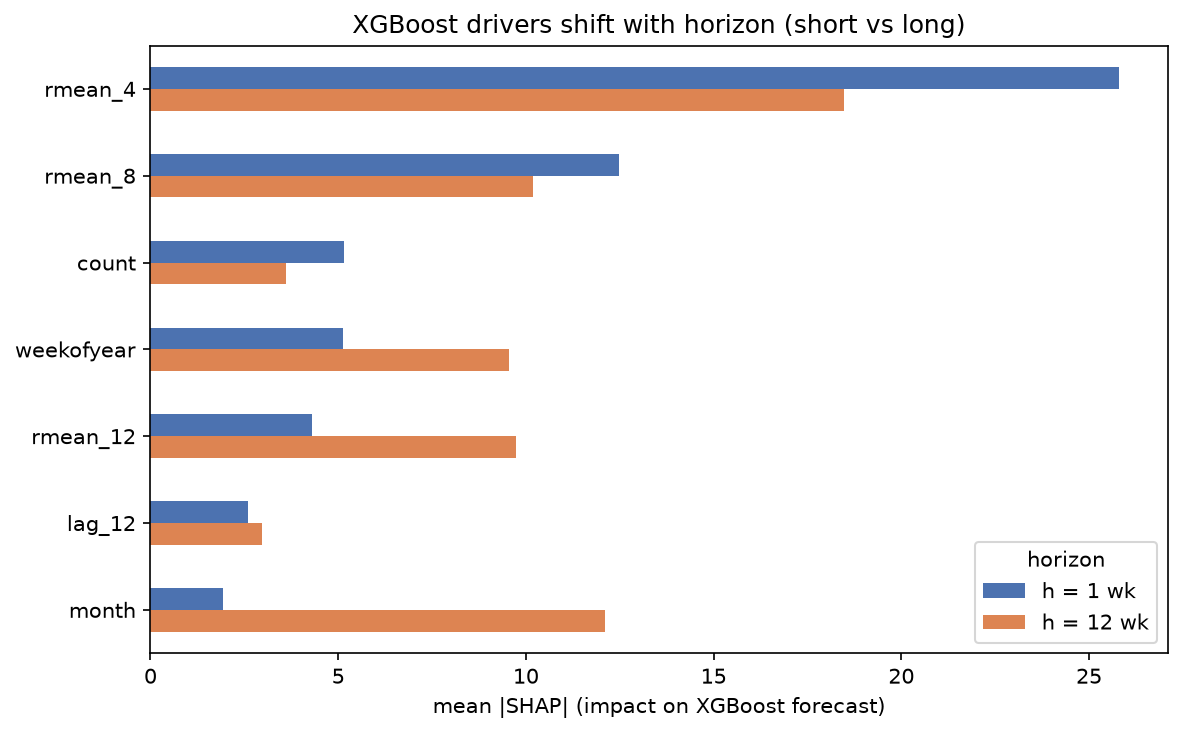
\includegraphics[width=0.78\linewidth]{fig_shap_by_horizon.png}
\caption{Mean $|$SHAP$|$ of the XGBoost member's top features at the shortest versus longest horizon:
recent rolling means dominate at $h{=}1$, while month/week-of-year grow at $h{=}12$.}
\label{fig:shaph}
\end{figure}

\section{Discussion}\label{sec:disc}
The consistent thread across our results is that the optimal forecaster mix is \emph{not constant}: it
shifts with horizon (Table~\ref{tab:weights}) and with regime (Fig.~\ref{fig:traj}). Combining models
significantly beats the best single model at all horizons, but---importantly and honestly---a simple
static inverse-RMSE blend is hard to beat in calm periods. The value of \emph{adaptive} weighting is
conditional: it is realised at the regime break, where the regime-adaptive scheme improves on the
static blend by 7--11\% and where, by contrast, the validation-fit horizon-adaptive scheme can overfit
its frozen weights. This is itself an argument for \emph{online} adaptation. Relative to the closest
prior art~\cite{ncaa2025}, which compares the same model family on the same data, our contribution is
the adaptive weighted combination (including the deep-learning member), the significance testing, and
the regime analysis. We deliberately do not pursue spatiotemporal deep-learning state of the art:
weekly district series are short ($\approx$500 points), favouring data-efficient, interpretable members,
and our question concerns the weighting mechanism rather than maximal accuracy.

\section{Ethics and Responsible Use}
Reported crime (CLEAR data) reflects enforcement and reporting behaviour, not underlying crime, and
carries feedback-loop risks. This work forecasts \emph{aggregate, district-level workload} for resource
planning---not individuals or specific locations. No demographic features are used and locations are
district-level only. The outputs should not be used for targeting decisions.

\section{Limitations and Future Work}
We study a single city at weekly resolution and do not include a spatial/graph member; per-crime-type
forecasting is left as a secondary analysis. The adaptive-weighting framework is, however,
member-agnostic: spatiotemporal models could be added as members, and the approach generalises to other
domains with structural breaks (e.g., energy demand, epidemiology).

\section{Conclusion}
We presented a horizon- and regime-adaptive weighted ensemble for multi-horizon, district-level crime
forecasting. The ensemble significantly beats the best single model at all horizons; the optimal mix
shifts with horizon and regime; and the advantage of adaptive over static weighting concentrates at the
2020 structural break. The practical message is that adaptivity pays \emph{when and where} the
data-generating regime shifts.

\begin{thebibliography}{9}
\bibitem{ncaa2025} Author(s). Exploratory data analysis, time series analysis, crime type prediction,
and trend forecasting in crime data using machine learning, deep learning, and statistical methods.
\emph{Neural Computing and Applications}, 2025. doi:10.1007/s00521-025-11094-9. % TODO: fill authors
\bibitem{chicago} City of Chicago. Crimes -- 2001 to Present, Chicago Data Portal, dataset ijzp-q8t2.
\bibitem{monteromanso2021} Montero-Manso P., Hyndman R.J. Principles and algorithms for forecasting
groups of time series: locality and globality. \emph{International Journal of Forecasting}, 37(4), 2021.
\bibitem{dm1995} Diebold F.X., Mariano R.S. Comparing predictive accuracy. \emph{J. Business \& Economic
Statistics}, 13(3), 1995.
\bibitem{prophet} Taylor S.J., Letham B. Forecasting at scale. \emph{The American Statistician}, 72(1),
2018.
\bibitem{xgboost} Chen T., Guestrin C. XGBoost: a scalable tree boosting system. \emph{KDD}, 2016.
\bibitem{shap} Lundberg S.M., Lee S.-I. A unified approach to interpreting model predictions.
\emph{NeurIPS}, 2017.
\bibitem{hyndman} Hyndman R.J., Athanasopoulos G. \emph{Forecasting: Principles and Practice}, 3rd ed.,
OTexts, 2021.
\end{thebibliography}

\end{document}
